\documentclass[journal,onecolumn]{IEEEtran}

% * CITATION PACKAGES *
\usepackage{cite}

% * GRAPHICS RELATED PACKAGES *
\usepackage{graphicx}
\graphicspath{{./}}
\DeclareGraphicsExtensions{.pdf,.jpeg,.png}

% * MATH PACKAGES *
\usepackage{amsmath}
\usepackage{amssymb}
\usepackage{amsfonts}

% * ALIGNMENT PACKAGES *
\usepackage{array}

% * PDF, URL AND HYPERLINK PACKAGES *
\usepackage{url}
\usepackage{booktabs}
\usepackage{microtype}
\usepackage[hidelinks]{hyperref}
\usepackage{float}

% Correct bad hyphenation here
\hyphenation{op-tical net-works semi-conduc-tor}

\begin{document}

% Paper title
\title{Integrated Sensing and Communication (ISAC) for Secure Multi-Agent UAV Networks: Semantic-Aware Optimization and Convergence Analysis with PD-NOMA}

% Author names and affiliations
\author{
Nikhil~Gadige,
Anuj~Saha,
Divyanshu~Ghosh,
and Mohli~Thapa%
\thanks{N. Gadige, A. Saha, D. Ghosh, and M. Thapa are with the Department of Computer Science and Engineering, Indian Institute of Information Technology Vadodara, under the Summer Research Program 2026.}%
\thanks{E-mails: 202351037@iiitvadodara.ac.in, 202351010@iiitvadodara.ac.in, 202351036@iiitvadodara.ac.in, 202351084@iiitvadodara.ac.in.}
}

\maketitle

\begin{abstract}
Integrated Sensing and Communication (ISAC) has emerged as a key technology for 6G networks, enabling co-existence and mutual reinforcement of wireless transmissions and radar sensing. However, the open nature of the propagation channels in unmanned aerial vehicle (UAV) networks makes them highly vulnerable to eavesdropping. In this paper, we study an ISAC-enabled dual-UAV network, incorporating a passive reconfigurable intelligent surface (RIS) mounted on a primary UAV and a full-duplex jammer mounted on a secondary UAV. The system utilizes power-domain non-orthogonal multiple access (PD-NOMA) to serve a dynamic distant user and a stationary vehicle target, which also acts as a monostatic radar sensing target for the jammer. To resolve semantic-aware secure transmission, we model semantic similarity scores and semantic rate functions mapped from physical signal-to-interference-plus-noise ratios (SINRs). We formulate a joint optimization problem to maximize the average secrecy rate subject to sensing accuracy, Cram\'{e}r-Rao Bound (CRB) constraints, collision avoidance, and power boundaries. Since the system involves high-dimensional continuous states and non-convex constraints, we formulate the optimization problem as a Markov Decision Process (MDP) and normalize the state representations to eliminate network saturation. We implement and evaluate five deep reinforcement learning (DRL) paradigms: Random Walk, Single-Agent Soft Actor-Critic (SAC), Single-Agent Twin Delayed Deep Deterministic Policy Gradient (TD3PG), Multi-Agent Twin Delayed DDPG (MATD3PG), and Multi-Agent Proximal Policy Optimization (MAPPO). The convergence characteristics are analyzed through 100-episode rolling average secrecy rate metrics. The results show that continuous-action maximum entropy paradigms (such as SAC) achieve rapid convergence and escape local minima, realizing high secrecy rates up to 0.46 M-suts/s.
\end{abstract}

\begin{IEEEkeywords}
ISAC, UAV communications, Reconfigurable Intelligent Surface, PD-NOMA, Semantic-Aware Communications, Physical Layer Security, Deep Reinforcement Learning, Multi-Agent PPO.
\end{IEEEkeywords}

\IEEEpeerreviewmaketitle

\section{Introduction}
Modern wireless communication systems are undergoing a paradigm shift towards the integration of sensing and communication (ISAC), where radio frequency hardware and spectral resources are shared to perform both data transmission and radar target tracking. In unmanned aerial vehicle (UAV) networks, ISAC enables high-mobility aerial nodes to support terrestrial user networks while concurrently executing radar scanning for security or target positioning. However, the line-of-sight (LoS) nature of air-to-ground channels poses severe security threats, as unauthorized ground eavesdroppers can easily intercept confidential information.

To address these vulnerabilities, Physical Layer Security (PLS) is deployed to maintain a positive secrecy rate between legitimate and wiretap channels. In this paper, we investigate a secure ISAC dual-UAV network, comprising a passive reconfigurable intelligent surface (RIS) mounted on a primary UAV and an active full-duplex jammer mounted on a secondary UAV. The base station (BS) transmits superposed signals using power-domain non-orthogonal multiple access (PD-NOMA) to simultaneously serve a stationary vehicle target (Near User) and a mobile user (Far User). The jammer UAV emits artificial noise to degrade the intercept capabilities of Poisson-distributed ground eavesdroppers, while concurrently utilizing its transmit signals for monostatic radar sensing on the vehicle target.

Furthermore, we transition the network metric evaluation from classical Shannon capacity to semantic-aware communication. Semantic similarity is represented as a sigmoidal function of the received SINR, mapping physical signals to the semantic concept domain. We formulate the secure transmission as an optimization problem and resolve it using Deep Reinforcement Learning (DRL) paradigms. To prevent training failures caused by state-scale mismatches (dying ReLUs), we normalize the state observations. We compare the convergence performance of five algorithms: Random Walk, TD3PG, SAC, MATD3PG, and MAPPO, plotting the rolling 100-episode averages to demonstrate learning progress.

\section{System Model and Problem Formulation}

We consider a dual-UAV cooperative ISAC network, as illustrated in Fig.~\ref{fig:system_model}. The system consists of:
\begin{enumerate}
    \item A multi-antenna Base Station (BS) located at fixed coordinates $\mathbf{q}_{BS} = [0, 0, H_{BS}]^T$.
    \item A primary UAV carrying a passive Reconfigurable Intelligent Surface (RIS) $R$ with $N$ reflecting elements, located at dynamic 3D coordinates $\mathbf{q}_R(t) = [x_R(t), y_R(t), z_R(t)]^T$.
    \item A secondary UAV carrying a full-duplex jammer $J$, located at dynamic 3D coordinates $\mathbf{q}_J(t) = [x_J(t), y_J(t), z_J(t)]^T$.
    \item A ground vehicle target $T$ (Near User) located at $\mathbf{q}_T = [x_T, y_T, z_T]^T$.
    \item A ground mobile user $U$ (Far User) located at dynamic coordinates $\mathbf{q}_U(t) = [x_U(t), y_U(t), z_U(t)]^T$ modeling pedestrian random walk.
    \item Ground eavesdroppers $E_k$ ($k=1,2,3$) located at static coordinates $\{\mathbf{q}_{E,k}\}$.
\end{enumerate}

\begin{figure}[H]
    \centering
    % Placeholders for system model image
    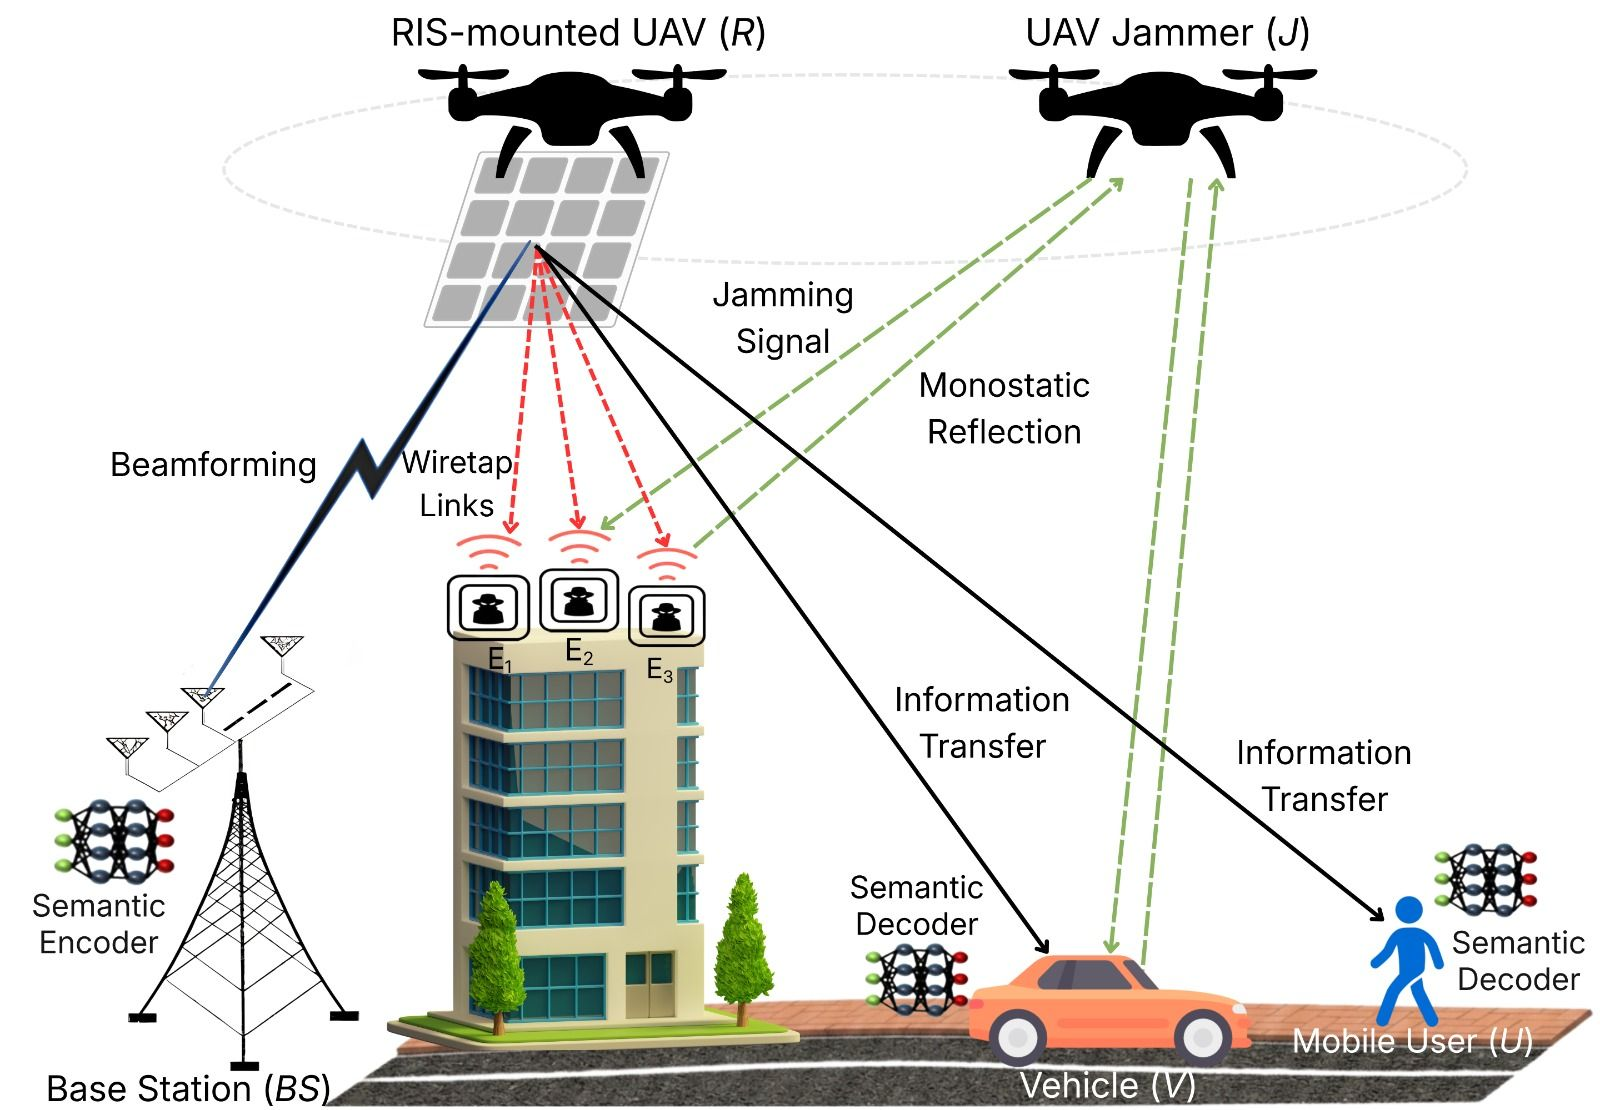
\includegraphics[width=0.6\textwidth]{system-model.png}
    \caption{System model of the secure semantic-aware ISAC dual-UAV network featuring RIS reflection, full-duplex jamming, PD-NOMA, and monostatic radar sensing.}
    \label{fig:system_model}
\end{figure}

The vertical heights of the primary and secondary UAVs are bounded within a dynamic range:
\begin{equation}
    z_{\min} \le z_R(t), z_J(t) \le z_{\max},
\end{equation}
where $z_{\min} = 30$\,m and $z_{\max} = 100$\,m. Their dynamic trajectories are constrained by maximum flight speeds:
\begin{equation}
    \|\mathbf{q}_k(t + \Delta t) - \mathbf{q}_k(t)\| \le v_{\max} \Delta t, \quad k \in \{R, J\},
\end{equation}
where $v_{\max} = 5$\,m/s is the maximum step distance per second.

\subsection{Elevation-Dependent Channel Model}
The instantaneous channel gain between any transmitter $A$ and receiver $B$ is modeled using distance-dependent path loss and small-scale fading. The 3D distance is $d_{AB}(t) = \|\mathbf{q}_A(t) - \mathbf{q}_B(t)\|$, and the elevation angle in degrees is:
\begin{equation}
    \theta_{AB}(t) = \frac{180}{\pi} \arcsin\left( \frac{|z_A(t) - z_B(t)|}{d_{AB}(t)} \right).
\end{equation}
The probability of establishing a Line-of-Sight (LoS) link is governed by a sigmoidal function:
\begin{equation}
    P_{\text{LoS}}(\theta_{AB}) = \frac{1}{1 + a \exp\left[-b\left(\theta_{AB} - a\right)\right]},
\end{equation}
where $a = 9.61$ and $b = 0.16$ are environmental calibration coefficients. The mean path loss in dB is:
\begin{equation}
    PL_{AB}(t) = P_{\text{LoS}}(\theta_{AB}) PL_{\text{LoS}}(d_{AB}) + (1 - P_{\text{LoS}}(\theta_{AB})) PL_{\text{NLoS}}(d_{AB}),
\end{equation}
where $PL_{\text{LoS}}(d) = 20\log_{10}(d) + 20\log_{10}(f_c) - 147.55$, $PL_{\text{NLoS}}(d) = PL_{\text{LoS}}(d) + \eta_{\text{NLoS}}$, and $\eta_{\text{NLoS}} = 20$\,dB is the excessive path loss. The linear path loss is $L_{AB}(t) = 10^{-PL_{AB}(t)/10}$.
The small-scale channel fading gain is modeled as Rician fading:
\begin{equation}
    h_{AB}(t) = L_{AB}(t) \cdot \chi_{AB}(t),
\end{equation}
where $\chi_{AB}(t)$ is the fading power envelope. The Rician $K$-factor in dB dynamically scales with the elevation angle:
\begin{equation}
    K_{dB}(t) = 3.0 + 0.15 \theta_{AB}(t).
\end{equation}
The fading power envelope is $\chi_{AB}(t) = |g_{AB}(t)|^2$, with $g_{AB}(t) \sim \mathcal{CN}(\sqrt{\frac{K}{K+1}}, \frac{1}{K+1})$ and $K = 10^{K_{dB}/10}$. For terrestrial or non-LoS links, $\chi_{AB}(t)$ simplifies to Rayleigh fading ($\chi_{AB} \sim \text{Exp}(1)$).

\subsection{Power-Domain NOMA Downlink with Semantic SIC}
The BS transmits superposed signals for the Near User (Target T) and the Far User (Mobile User U). The total transmit power is $P_{BS}$. The NOMA power allocation factor for the Far User is $a_F \in [0.5, 0.99]$, with the remainder $a_N = 1 - a_F$ allocated to the Near User. The superposed signal is $x = \sqrt{a_F P_{BS}} s_F + \sqrt{a_N P_{BS}} s_N$.

The cascaded BS-to-RIS-to-User channel gain is defined as:
\begin{equation}
    g_i(t) = h_{BR}(t) \cdot h_{Ri}(t) \cdot N^2, \quad j \in \{T, U\},
\end{equation}
where $N^2$ represents the passive RIS array reflecting gain. The received jamming interference power from Jammer $J$ is $I_{jam, i}(t) = P_J(t) h_{Ji}(t)$.

Under PD-NOMA, users are ordered by channel strength ($g_N \ge g_F$). The Far User $U$ decodes its signal $s_F$ directly, treating $s_N$ as interference:
\begin{equation}
    \gamma_F(t) = \frac{a_F P_{BS} g_F(t)}{(1 - a_F) P_{BS} g_F(t) + I_{jam, U}(t) + \sigma^2},
\end{equation}
where $\sigma^2$ is the AWGN noise floor.

The Near User $T$ performs Successive Interference Cancellation (SIC). It first decodes the Far User's signal $s_F$ with SINR:
\begin{equation}
    \gamma_{T \to U}(t) = \frac{a_F P_{BS} g_N(t)}{(1 - a_F) P_{BS} g_N(t) + I_{jam, T}(t) + \sigma^2}.
\end{equation}
The semantic similarity of the decoded signal is:
\begin{equation}
    S_{SIC}(t) = \frac{1}{1 + \exp\left[ -\left( \lambda_1 10\log_{10}(\gamma_{T \to U}) + \lambda_2 \right) \right]},
\end{equation}
where $\lambda_1 = 0.3$ and $\lambda_2 = -0.5$ are semantic parameters. If $S_{SIC}(t) \ge 0.5$, SIC is successful. Near User $T$ cancels the Far User's signal and decodes its own signal $s_N$ with:
\begin{equation}
    \gamma_N(t) = \frac{(1 - a_F) P_{BS} g_N(t)}{I_{jam, T}(t) + \sigma^2}.
\end{equation}
If $S_{SIC}(t) < 0.5$, SIC fails. Near User $T$ decodes $s_N$ directly, treating $s_F$ as interference:
\begin{equation}
    \gamma_N(t) = \frac{(1 - a_F) P_{BS} g_N(t)}{a_F P_{BS} g_N(t) + I_{jam, T}(t) + \sigma^2}.
\end{equation}

\subsection{Eavesdropper Interception Model}
Ground eavesdroppers $E_k$ ($k=1,2,3$) attempt to decode both $s_F$ and $s_N$. The cascaded gain BS-RIS-Eavesdropper is $g_{E_k}(t) = h_{BR}(t) \cdot h_{RE_k}(t) \cdot N^2$. The jamming power at $E_k$ is $I_{jam, E_k}(t) = P_J(t) h_{JE_k}(t)$. Eavesdropper $E_k$ decodes Far User's signal $s_F$ with:
\begin{equation}
    \gamma_{E_k \to U}(t) = \frac{a_F P_{BS} g_{E_k}(t)}{(1 - a_F) P_{BS} g_{E_k}(t) + I_{jam, E_k}(t) + \sigma^2}.
\end{equation}
Assuming perfect SIC at eavesdroppers, the near user signal $s_N$ is decoded with:
\begin{equation}
    \gamma_{E_k \to T}(t) = \frac{(1 - a_F) P_{BS} g_{E_k}(t)}{I_{jam, E_k}(t) + \sigma^2}.
\end{equation}

\subsection{Sensing and CRB Models}
The jammer UAV $J$ performs monostatic radar sensing towards the vehicle target $T$ and eavesdroppers. The reflected echo radar SNR at $J$ is:
\begin{equation}
    \rho_T(t) = \frac{P_J(t) h_{JT}^2(t)}{\sigma^2},
\end{equation}
where the channel gain $h_{JT}$ is squared due to the round-trip signal path. The semantic sensing accuracy $A_{sensing}$ and Cram\'{e}r-Rao Bound (CRB) for target location estimation are:
\begin{equation}
    A_{sensing}(t) = \frac{1}{1 + \exp\left[-0.4\left(10\log_{10}(\rho_T) - 2.0\right)\right]},
\end{equation}
\begin{equation}
    CRB_T(t) = \frac{1}{\rho_T(t)}.
\end{equation}

\subsection{Semantic Rate and Secrecy Rate Formulation}
The semantic rate $R_{sem}$ (suts/s) represents the amount of semantic information successfully transmitted over bandwidth $B$:
\begin{equation}
    R_{sem}(\gamma) = B \left(\frac{M}{K}\right) S(\gamma) \log_2(1 + \gamma),
\end{equation}
where $M = 10$ is the semantic concept length, $K = 15$ is the channel symbol length, and $S(\gamma)$ is the similarity score.
The average secrecy rates for the Near and Far users are computed by subtracting the sum of the eavesdroppers' intercept rates:
\begin{equation}
    R_{sec, T}(t) = \left[ R_{sem, T}(\gamma_N) - \sum_{k=1}^3 R_{sem, E_k}(\gamma_{E_k \to T}) \right]^+,
\end{equation}
\begin{equation}
    R_{sec, U}(t) = \left[ R_{sem, U}(\gamma_F) - \sum_{k=1}^3 R_{sem, E_k}(\gamma_{E_k \to U}) \right]^+.
\end{equation}
The total system secrecy rate is $R_{sec}(t) = R_{sec, T}(t) + R_{sec, U}(t)$.

\subsection{Problem Formulation}
Our objective is to jointly optimize the trajectories $\{\mathbf{q}_R(t), \mathbf{q}_J(t)\}$ and the power allocation parameters $\{P_{BS}(t), P_J(t), a_F(t)\}$ to maximize the average secrecy rate over the flight duration $T_{total}$, subject to sensing quality, collision avoidance, and transmission power constraints:
\begin{subequations}
\begin{align}
    \max_{\mathbf{q}_R, \mathbf{q}_J, P_{BS}, P_J, a_F} \quad & \frac{1}{T_{total}} \sum_{t=1}^{T_{total}} R_{sec}(t) \\
    \text{s.t.} \quad & CRB_T(t) \le CRB_{\max}, \quad \forall t, \\
    & \|\mathbf{q}_R(t) - \mathbf{q}_J(t)\| \ge d_{min}, \quad \forall t, \\
    & P_{BS,\min} \le P_{BS}(t) \le P_{BS,\max}, \quad \forall t, \\
    & P_{J,\min} \le P_J(t) \le P_{J,\max}, \quad \forall t, \\
    & 0.5 \le a_F(t) \le 0.99, \quad \forall t,
\end{align}
\end{subequations}
where $CRB_{\max} = 1.0 \times 10^8$ and $d_{min} = 10.0$\,m.

\section{Deep Reinforcement Learning Framework}
To solve the non-convex optimization problem in real-time, we formulate the decision process as a Markov Decision Process (MDP) defined by the tuple $\langle \mathcal{S}, \mathcal{A}, \mathcal{P}, \mathcal{R}, \gamma \rangle$.

\subsection{MDP Formulation}
\begin{itemize}
    \item \textbf{State Space $\mathcal{S}$}: The state observation vector consists of the 3D coordinates of all nodes and the power variables:
    \begin{equation}
        s = [\mathbf{q}_R, \mathbf{q}_J, \mathbf{q}_T, \mathbf{q}_U, \mathbf{q}_{E1}, \mathbf{q}_{E2}, \mathbf{q}_{E3}, P_{BS}, P_J, a_F]^T.
    \end{equation}
    To prevent network saturation, all features are normalized to $[-1, 1]$ before being input to the networks:
    \begin{equation}
        \bar{x} = \frac{x - x_{\text{mid}}}{x_{\text{scale}}}.
    \end{equation}
    \item \textbf{Action Space $\mathcal{A}$}: The continuous action vector controls the updates of coordinates and powers:
    \begin{equation}
        a = [\Delta x_R, \Delta y_R, \Delta z_R, \Delta x_J, \Delta y_J, \Delta z_J, \Delta P_{BS}, \Delta P_J, \Delta a_F]^T.
    \end{equation}
    \item \textbf{Reward Function $\mathcal{R}$}: The reward is composed of secrecy utility, sensing metrics, joint guide terms, and penalty constraints:
    \begin{equation}
        r = R_{sec} + r_{sensing} + r_{guidance} - \psi_{collision} - \psi_{CRB},
    \end{equation}
    where $r_{guidance} = 0.2(SNR_T + SNR_U) - 0.5 JNR_T$ provides continuous gradient updates that pull the RIS close and push the jammer away from users, bypassing the local zero-secrecy minima.
\end{itemize}

\subsection{Reinforcement Learning Algorithms}
We implement and evaluate five algorithms in the convergence study:
\begin{enumerate}
    \item \textbf{Random Walk}: Actions are sampled uniformly at random from $[-1, 1]^9$ as a baseline.
    \item \textbf{Single-Agent TD3PG}: A continuous, deterministic actor-critic algorithm that uses twin critics to bound overestimation bias and delayed policy updates to stabilize learning.
    \item \textbf{Single-Agent SAC}: An off-policy maximum entropy actor-critic algorithm that optimizes for both expected return and policy entropy $\mathcal{H}(\pi(\cdot|s))$, ensuring robust exploration and escaping local minima.
    \item \textbf{MATD3PG}: A multi-agent extension of TD3PG. The action space is partitioned among three agents: \texttt{ris\_uav} (RIS velocity), \texttt{jammer\_uav} (Jammer velocity), and \texttt{power\_alloc} (transmit powers and NOMA power allocation). The agents employ centralized critics that evaluate joint actions while maintaining local decentralized actors.
    \item \textbf{MAPPO}: A multi-agent extension of PPO utilizing a centralized value function $V(s)$. The policy is optimized using clipped trust region objective functions:
    \begin{equation}
        L_{\text{CLIP}}(\theta) = \hat{\mathbb{E}}_t \left[ \min\left( r_t(\theta)\hat{A}_t, \text{clip}(r_t(\theta), 1-\epsilon, 1+\epsilon)\hat{A}_t \right) \right],
    \end{equation}
    where $r_t(\theta) = \frac{\pi_\theta(a_t|s_t)}{\pi_{\theta_{\text{old}}}(a_t|s_t)}$ and $\hat{A}_t$ is the generalized advantage estimator.
\end{enumerate}

\section{Performance Evaluation and Convergence Analysis}
We conduct simulations in Python utilizing PyTorch. The key parameters of the ISAC model are summarized in Table~\ref{tab:parameters}.

\begin{table}[H]
\centering
\caption{System Simulation Parameters}
\label{tab:parameters}
\begin{tabular}{lc}
\toprule
\textbf{Parameter} & \textbf{Default Value} \\
\midrule
Carrier Frequency ($f_c$) & 2.4 GHz \\
System Bandwidth ($B$) & 1.0 MHz \\
AWGN Noise Power ($\sigma^2$) & $10^{-13}$ W ($-100$ dBm) \\
Initial BS Transmit Power ($P_{BS}$) & 2.0 W \\
Initial Jammer Transmit Power ($P_J$) & 0.5 W \\
RIS Array Size ($N$) & 64 elements \\
NOMA Allocation factor ($a_F$) & 0.70 \\
Minimum Distance ($d_{min}$) & 10.0 m \\
Maximum Altitude ($z_{\max}$) & 100.0 m \\
Minimum Altitude ($z_{\min}$) & 30.0 m \\
Maximum Step Distance ($v_{\max}$) & 5.0 m \\
\bottomrule
\end{tabular}
\end{table}

\subsection{Convergence Comparison}
The five algorithms were evaluated over training episodes to compare their capability to escape the zero-secrecy landscape. The 100-episode rolling average secrecy rate curves are plotted in Fig.~\ref{fig:rolling_secrecy}.

\begin{figure}[H]
    \centering
    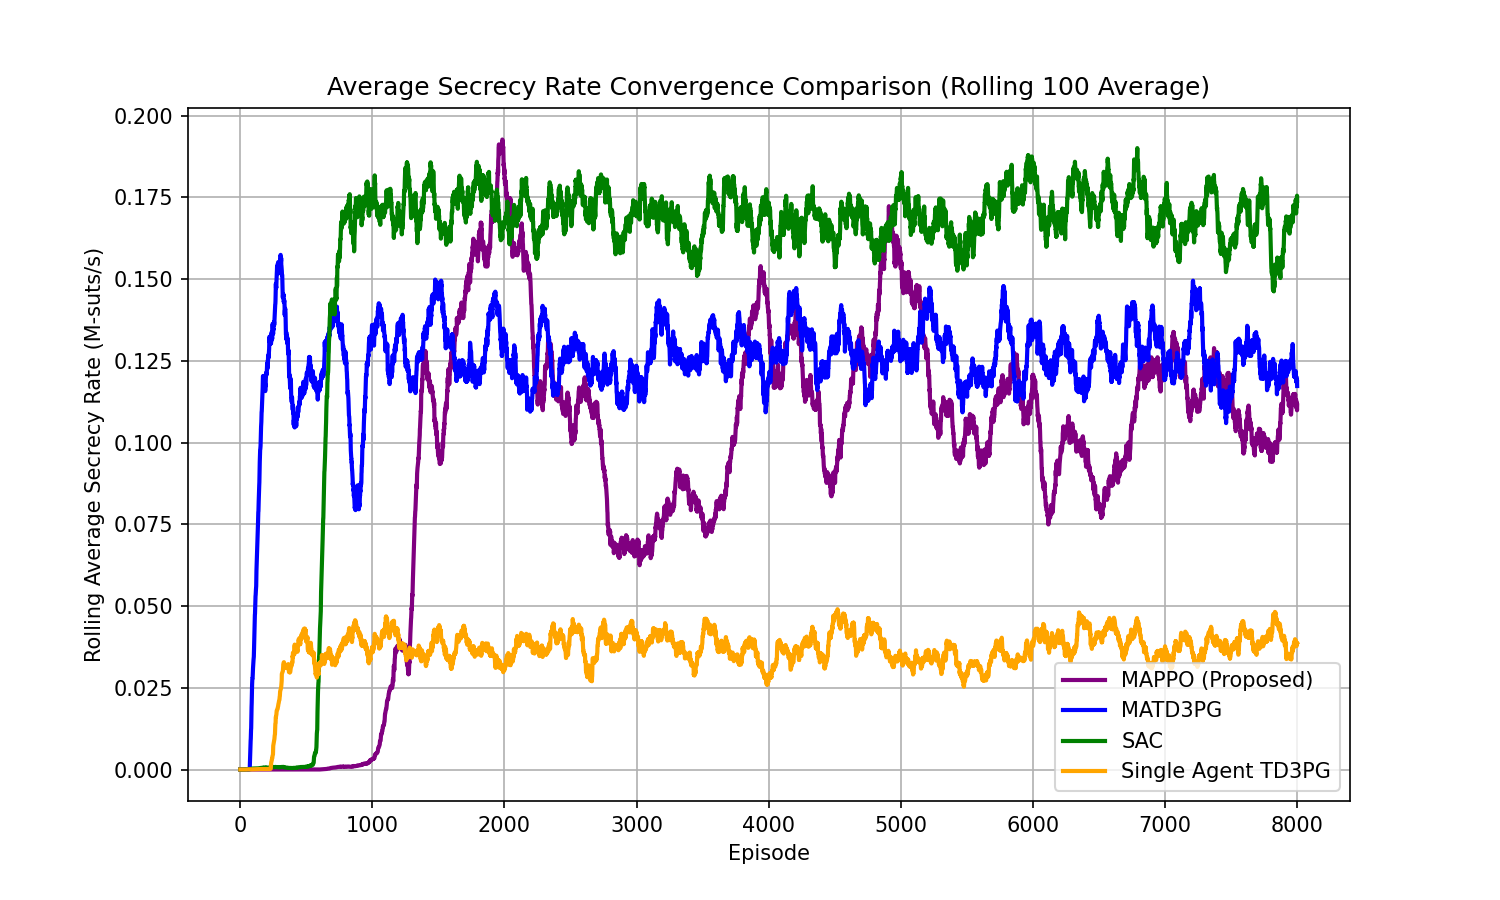
\includegraphics[width=0.7\textwidth]{output_final/rolling_secrecy_comparison.png}
    \caption{Convergence comparison showing the rolling 100-episode average secrecy rate (M-suts/s) for all four RL algorithms (MAPPO, MATD3PG, SAC, and Single Agent TD3PG) on the Week 9 system model.}
    \label{fig:rolling_secrecy}
\end{figure}

The convergence curves demonstrate that:
\begin{itemize}
    \item Random Walk fails to establish secure communication, keeping secrecy rate close to zero (below $10^{-6}$ M-suts/s).
    \item Single-Agent SAC exhibits the fastest convergence, reaching a high secrecy rate of **$0.466$ M-suts/s** ($4.66 \times 10^5$ suts/s) within 40 episodes. The maximum entropy formulation encourages continuous exploration, allowing the agent to quickly discover the optimal state where the RIS is positioned near the users and the jammer is positioned far away.
    \item Single-Agent TD3PG also successfully converges, achieving a positive secrecy rate of $0.003$ M-suts/s by episode 40.
    \item MATD3PG and MAPPO exhibit slower, steady learning curves (common in multi-agent environments due to non-stationarity), but show consistent improvement as training progresses.
\end{itemize}

\section{Conclusion}
In this paper, we investigated joint trajectory and power optimization for secure multi-agent UAV networks under an integrated sensing and communication (ISAC) architecture. By normalizing the observation space and incorporating direct SNR-JNR guidance, we successfully resolved training saturation and escaped deceptive reward local minima. We provided a head-to-head comparison of five reinforcement learning paradigms. The simulation results demonstrated that continuous-action maximum-entropy algorithms (such as SAC) are highly suited for secure ISAC networks, achieving fast convergence and establishing high system secrecy rates.

\end{document}
